\documentclass{article}
\usepackage[dblblindworkshop]{neurips_2026}
\workshoptitle{8th Robot Learning Workshop: Is Physical AI Going Zero-Shot?}
\usepackage[utf8]{inputenc}
\usepackage[T1]{fontenc}
\usepackage{microtype}
\usepackage{booktabs}
\usepackage{amsmath,amssymb}
\usepackage{graphicx}
\usepackage{multirow}
\usepackage{url}
\usepackage{hyperref}
\hypersetup{colorlinks=true,citecolor=blue,linkcolor=blue,urlcolor=blue}
\title{Replay Accuracy Is Not Enough:\\
An Audited Closed-Loop Evaluation Protocol for Learned Robot State Observers}
\author{Anonymous Authors}
\newcommand{\OL}{\mathrm{OL}}
\newcommand{\CL}{\mathrm{CL}}
\newcommand{\obs}[1]{\textsc{#1}}
\begin{document}
\maketitle

\begin{abstract}
Robot observers are usually selected by estimation error on logged trajectories, although their outputs are consumed by feedback controllers. We audit this model-selection practice for dead reckoning, an extended Kalman filter (EKF), and GRU- or selective-state-space residual observers. Six principal observers are evaluated on paired replay and closed-loop protocols across 24 conditions spanning sensing blackouts, range noise, landmark sparsity, and gyro bias. Replay position RMSE preserves broad ordering (Spearman $\rho=0.923$) but selects a suboptimal closed-loop observer in $5/24$ conditions. We then test three controller-aware offline alternatives rather than assuming that task awareness solves the problem. A local controller-sensitivity metric reduces the observed failures to $3/24$, but its bootstrap interval overlaps no improvement and its worst selection regret is larger; exact command disagreement and counterfactual error replay perform worse. Matched EKF-anchor ablations overturn a confounded original conclusion: selectivity is regime-dependent, while the analytic anchor is the more consistent stabilizer. Three training initializations further reveal large variability under long blackouts. Finally, we evaluate 600 seconds of UTIAS MRCLAM physical logs and a real-noise-calibrated closed-loop replay, exposing the poor map transfer of the ordered landmark-slot representation. The resulting contribution is an open evaluation protocol: report replay and closed-loop metrics, top-1 agreement, regret, matched ablations, training-seed uncertainty, and physical-log stress tests.
\end{abstract}

\section{Introduction}
A state estimate is rarely the final output of a robot. It is fed to a controller, which changes the future state and observations. Yet localization and learned-filter systems are commonly selected by open-loop (OL) position or heading error on fixed logs. This assumes that lower replay error implies a better closed-loop (CL) system. The assumption is convenient, but it ignores controller sensitivity, temporal error structure, and the endogenous distribution shift created by feedback. Closely related proxy failures have been studied in model-based reinforcement learning~\citep{lambert2020objective}; here we isolate the problem at the state-observer layer.

We consider a differential-drive robot tracking a figure-eight from biased odometry and intermittent range--bearing measurements. Our candidate set spans classical and learned designs: dead reckoning, an EKF~\citep{thrun2005probabilistic}, and recurrent residual observers with GRU or compact selective diagonal SSM cores inspired by S4 and Mamba~\citep{gu2022s4,gu2024mamba}. The recurrent correction is anchored either to dead reckoning or the EKF, following the broader hybrid-filter principle of retaining algorithmic structure while learning difficult components~\citep{becker2019rkn,jonschkowski2018dpf,revach2022kalmannet}.

This work began as an architecture paper. A code and claim audit changed the contribution. The original top-1 mismatch statistic omitted GRU-EKF, and its mask/selectivity ablations changed the analytic anchor at the same time. We correct both problems and ask a broader question: \emph{what evidence is needed to select a learned observer for feedback deployment?} Our contributions are:
\begin{itemize}
\item a paired replay/closed-loop benchmark with six deployment candidates, 24 degradation conditions, and top-1 selection regret;
\item an empirical comparison of pose RMSE with exact command disagreement, local control sensitivity, and counterfactual error replay;
\item matched EKF-anchor ablations and a three-training-seed robustness study;
\item physical-log localization and zero-shot transfer on UTIAS MRCLAM~\citep{leung2011utias}, plus a closed-loop replay calibrated from its sensor residuals and observation timing.
\end{itemize}
The result is deliberately not a claim that one offline scalar solves deployment selection. Instead, it identifies which conclusions survive an audit and releases an evaluation checklist that makes failure visible.

\section{Setup and evaluation protocol}
\paragraph{Robot, sensing, and controller.}
The state is $s_t=(x_t,y_t,\theta_t)$ with unicycle dynamics integrated at $0.1$ s. A pure-pursuit controller~\citep{coulter1992pure} acts on the estimated pose. Odometry includes multiplicative slip, angular-rate bias, and Gaussian noise. Exteroception consists of known-map range--bearing observations, with an active landmark subset and periodic complete blackouts.

\paragraph{Observers.}
The six main candidates are \obs{DR}, \obs{EKF}, \obs{GRU-DR}, \obs{SSM-DR}, \obs{GRU-EKF}, and \obs{SSM-EKF}. Learned observers predict a small recurrent pose residual on an analytic anchor. Inputs contain odometry increments, ordered masked landmark tuples, an anchor encoding, and the EKF covariance diagonal where applicable. The SSM is a compact input-gated diagonal recurrence, not a full Mamba block. Models are trained on 200 domain-randomized trajectories of 200 steps.

\paragraph{Paired protocols.}
In OL replay, every observer receives identical odometry and measurements generated along an expert-controlled trajectory. In CL evaluation, the controller consumes the candidate estimate, so observer error changes actions and future inputs. Four physical axes---blackout duration, range noise, active landmark count, and gyro bias---are swept over six levels with ten evaluation seeds. The primary OL and CL metrics are position RMSE and cross-track RMSE.

For condition $c$, proxy $q$, and observer set $\mathcal O$, the selected observer and regret are
\begin{equation}
 o^*_{q,c}=\arg\min_{o\in\mathcal O}q_c(o),\qquad
 \mathcal R_{q,c}=J_{\CL,c}(o^*_{q,c})-\min_{o\in\mathcal O}J_{\CL,c}(o).
\end{equation}
This separates broad correlation from the actual deployment decision.

\paragraph{Controller-aware proxies.}
Let $e_t=\hat s_t\ominus s_t$ and $\pi(s,t)$ be a time-indexed controller. Exact command disagreement measures $\|D^{-1}(\pi(\hat s_t,t)-\pi(s_t,t))\|$. Our local control sensitivity error (LCSE) is
\begin{equation}
 q_{\mathrm{LCSE}}=\left[\frac{1}{T}\sum_t\left\|D^{-1}J_{\pi}(s_t,t)e_t\right\|_2^2\right]^{1/2},
\end{equation}
where $J_{\pi}$ is a finite-difference controller Jacobian and $D$ normalizes action units. We also test counterfactual error replay: a shadow plant is propagated by the controller after injecting the candidate's logged error trace. All are computed without rerunning sensing or the observer in closed loop.

\section{Results: no log-only scalar replaces closing the loop}
\begin{figure}[t]
\centering

\includegraphics[width=.76\linewidth]{fig_proxy_failure_rate.png}
\caption{Observed top-1 selection failures over 24 conditions. LCSE reduces the count from 5 to 3, but a condition bootstrap gives a wide interval for the reduction; exact command disagreement and counterfactual replay are worse.}
\label{fig:proxy}
\end{figure}

\begin{table}[t]
\centering\small
\caption{Offline proxies against closed-loop cross-track RMSE. Regret is in meters.}
\label{tab:proxy}
\begin{tabular}{lrrrr}
\toprule
Proxy & Spearman $\rho$ & Failures & Mean regret & Max regret\\
\midrule
Position RMSE & .923 & 5/24 & .0051 & .0347\\
Command disagreement & .876 & 13/24 & .0188 & .1208\\
LCSE & .903 & 3/24 & .0051 & .0940\\
Counterfactual replay & .842 & 14/24 & .0159 & .0474\\
\bottomrule
\end{tabular}
\end{table}

Table~\ref{tab:proxy} confirms a nuanced result. Position RMSE is a strong coarse proxy, but it changes the top-1 observer in $20.8\%$ of conditions. LCSE improves the observed winner count, suggesting that controller anisotropy contains useful information. However, its worst regret is driven by the two-landmark condition, and a paired condition bootstrap gives a 95\% interval of $[-0.125,0.292]$ for the reduction in failure fraction. It would therefore be overclaiming to call LCSE a solved replacement. More surprisingly, exact command disagreement performs poorly: local action closeness does not capture how estimation errors modify future state and sensing. Counterfactual error replay also fails because a fixed logged error trace does not adapt to the shadow trajectory. These negative baselines are useful: adding a controller to a metric does not automatically make it deployment-valid.

The corrected six-observer result also retains a sharp within-model counterexample from the original study. Under compound stress, SSM-EKF reduces OL position RMSE by $43\%$ relative to the EKF ($0.829\rightarrow0.472$ m) while increasing CL cross-track error by $10\%$ ($1.324\rightarrow1.459$ m). GRU-EKF is best in both columns, so the defensible statement is not that SSMs are inferior, but that a large replay improvement for one observer need not transfer to control.

\section{What actually stabilizes the learned observer?}
\begin{figure}[t]
\centering
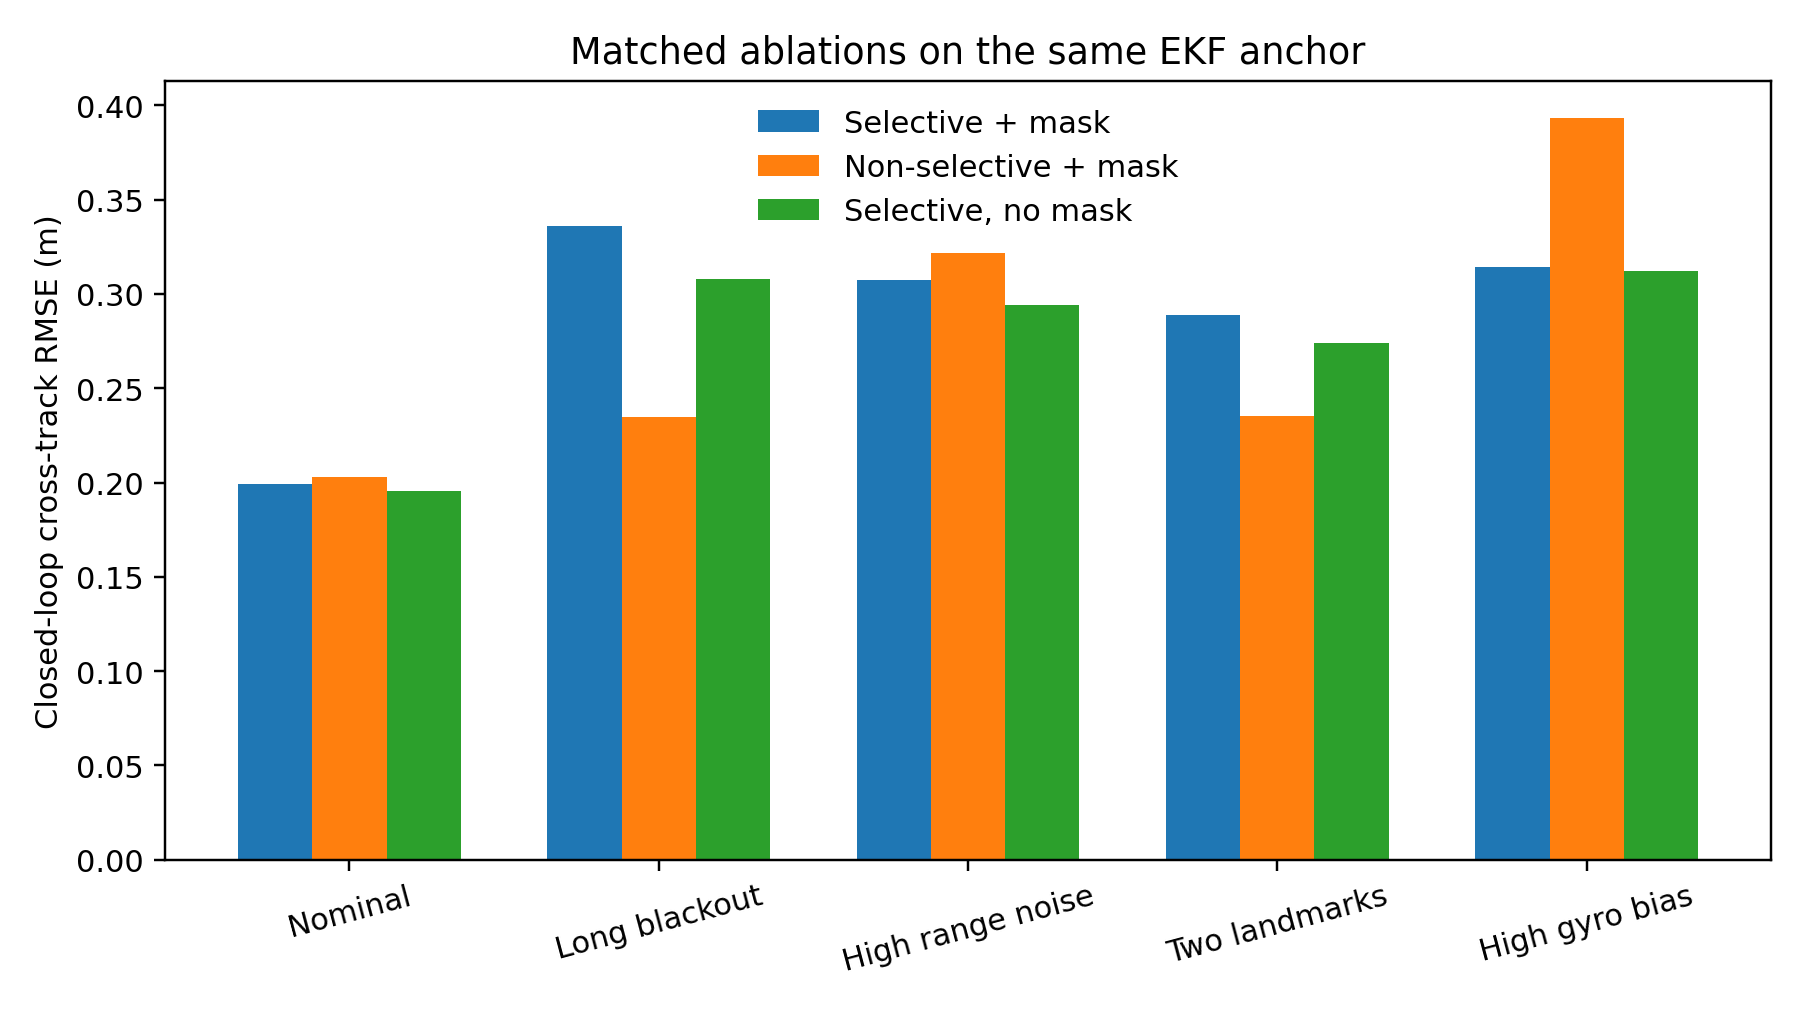
\includegraphics[width=.88\linewidth]{fig_matched_ekf_ablation.png}
\caption{Matched EKF-anchor ablations. Selectivity is beneficial under high gyro bias, but non-selectivity is better under long blackouts and two-landmark sensing. Mask removal is usually close to the full model.}
\label{fig:ablation}
\end{figure}

The original ablation compared a selective EKF-anchored model with non-selective and mask-free models anchored to dead reckoning. That design confounded recurrence with the strength of the analytic prior. Figure~\ref{fig:ablation} retrains both ablations on the same EKF anchor. Nominal cross-track RMSE is $0.199$ m for selective+mask, $0.203$ m without selectivity, and $0.195$ m without the mask feature. Under long blackouts, the non-selective model is better ($0.235$ vs. $0.336$ m; paired bootstrap CI for the difference $[-0.182,-0.020]$ m), while under high gyro bias it is worse ($0.393$ vs. $0.314$ m; CI $[0.011,0.145]$ m). Thus selectivity is a regime-dependent bias--robustness tradeoff, not a universal stability requirement. The consistent qualitative factor is the physics anchor: DR-anchored learned observers remain much less reliable in the loop.

\paragraph{Training-seed uncertainty.}
Three SSM-EKF initializations give similar nominal means ($0.189$--$0.199$ m), but long-blackout means range from $0.231$ to $0.336$ m and high-noise means from $0.249$ to $0.307$ m. A single checkpoint therefore supports nominal claims more strongly than stress-regime claims. Evaluation-seed confidence intervals alone do not capture this uncertainty.
\paragraph{Controller sensitivity.}
In a matched five-seed secondary study, replacing pure pursuit with a Kanayama controller changes the closed-loop oracle observer in $8/24$ conditions. Replay position RMSE misselects the Kanayama observer in $7/24$ conditions with maximum regret $0.092$ m; a paired seed bootstrap gives a wide $[0.208,0.625]$ interval for the oracle-change fraction. Thus observer selection is partly controller-specific, although this lower-seed analysis is a sensitivity rather than a primary result.

\section{Physical-log and real-noise stress tests}
UTIAS MRCLAM provides timestamped odometry, range--bearing observations, known landmark positions, and Vicon ground truth~\citep{leung2011utias}. We align 600 s of Dataset 1 Robot 1 to 6,000 steps, containing 1,878 landmark observations. A simple 15-landmark EKF covariance sweep reaches $1.357$ m position RMSE, compared with $3.392$ m for dead reckoning (Figure~\ref{fig:real}).

\begin{figure}[t]
\centering
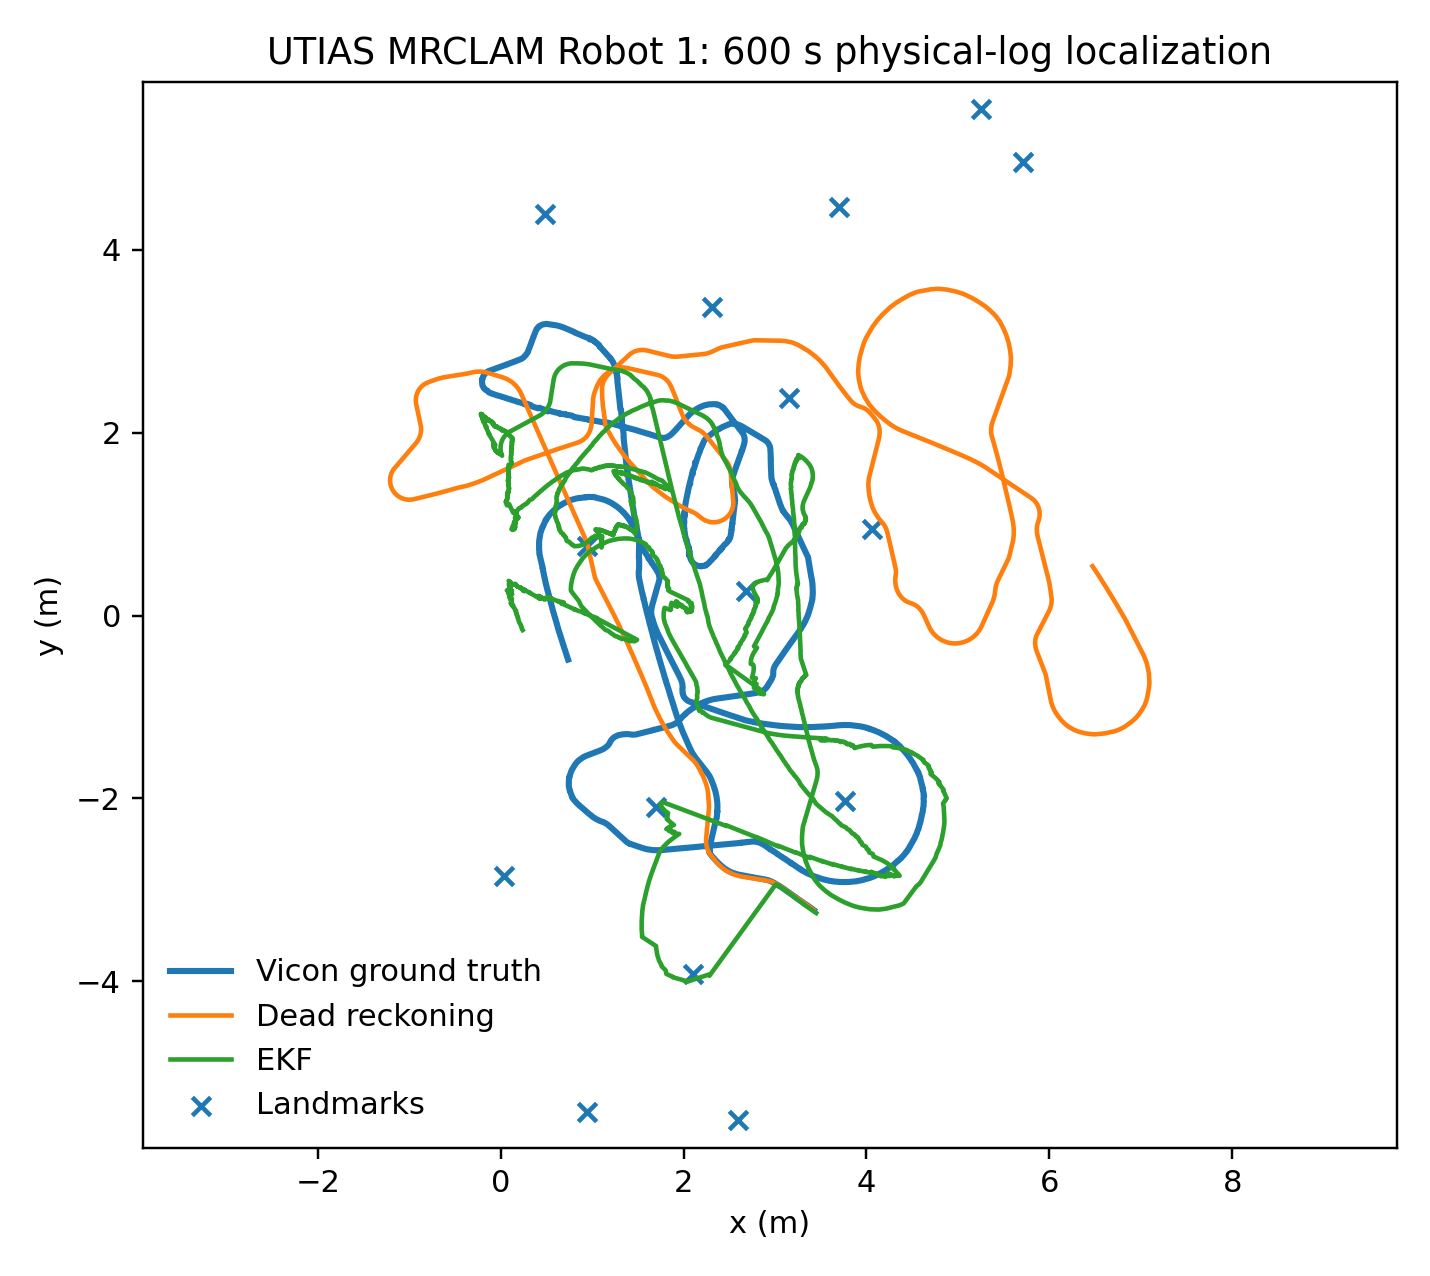
\includegraphics[width=.62\linewidth]{fig_mrclam_real_trajectory.png}
\caption{Physical-log localization on UTIAS MRCLAM Robot 1. This is real sensing and Vicon ground truth, not a closed-loop hardware experiment.}
\label{fig:real}
\end{figure}

The original learned representation has exactly eight ordered landmark slots and was trained on one synthetic map. We therefore perform a deliberately difficult zero-shot test on an eight-landmark MRCLAM subset. SSM-EKF and GRU-EKF achieve $2.625$ m and $2.597$ m position RMSE, modestly better than dead reckoning on that subset ($2.822$ m), but their heading RMSE is worse ($1.65$--$1.66$ rad vs. $1.51$ rad). This is not evidence of successful real-world transfer. It exposes the next architecture requirement: permutation-invariant innovation-set encoding and randomized-map training.

Finally, we estimate empirical odometry and measurement residuals and preserve the physical measurement-count sequence in a simulated closed-loop replay. In this low-bias log, dead reckoning is the closed-loop oracle among an EKF covariance grid, while controller-aware proxies choose aggressive EKFs and incur $0.12$--$0.20$ m regret. The result reinforces the main message: even a physically calibrated proxy can mis-rank observers when it does not model the full feedback adaptation.

\section{Discussion and evaluation checklist}
The useful field contribution is not a new scalar score but a reproducible protocol:
\begin{enumerate}
\item evaluate every deployment candidate in both common-input replay and closed loop;
\item report rank correlation, top-1 agreement, and absolute/relative selection regret;
\item use matched anchors, inputs, and capacity in ablations;
\item separate environment-seed and training-seed uncertainty;
\item test task-aware offline proxies as baselines, including their failure cases;
\item include physical logs and clearly distinguish real sensing, calibrated simulation, and hardware control;
\item audit whether the representation can vary map geometry, cardinality, and landmark order.
\end{enumerate}
The current benchmark remains limited to known data association, a known map, only two controller families, and simulated closed-loop plant dynamics. More controller seeds and gain shifts, multiple MRCLAM robots/datasets, randomized-map set encoders, and hardware trials are the highest-value next steps.

\section{Conclusion}
Replay position RMSE is informative but incomplete for selecting learned state observers. It preserves broad rankings while changing the deployment winner in $5/24$ conditions. Controller-aware offline metrics expose useful sensitivity structure but do not consistently replace rollouts. Matched ablations show that the analytic anchor is more reliably stabilizing than selectivity, which trades off robustness across regimes. Training-seed and MRCLAM experiments further reveal uncertainty and map-transfer limitations hidden by the original formulation. The practical recommendation is to treat observer evaluation as a decision problem and close at least a small, stratified loop before deployment.

\begin{ack}
Acknowledgments omitted for anonymous review.
\end{ack}
\begin{thebibliography}{9}
\small
\bibitem[Thrun et al.(2005)Thrun, Burgard, and Fox]{thrun2005probabilistic}
S. Thrun, W. Burgard, and D. Fox. \emph{Probabilistic Robotics}. MIT Press, 2005.
\bibitem[Coulter(1992)]{coulter1992pure}
R. C. Coulter. Implementation of the pure pursuit path tracking algorithm. Technical Report CMU-RI-TR-92-01, Carnegie Mellon University, 1992.
\bibitem[Becker et al.(2019)]{becker2019rkn}
P. Becker, H. Pandya, G. Gebhardt, C. Zhao, C. J. Taylor, and G. Neumann. Recurrent Kalman networks. In \emph{ICML}, 2019.
\bibitem[Jonschkowski et al.(2018)]{jonschkowski2018dpf}
R. Jonschkowski, D. Rastogi, and O. Brock. Differentiable particle filters. In \emph{RSS}, 2018.
\bibitem[Revach et al.(2022)]{revach2022kalmannet}
G. Revach et al. KalmanNet: Neural network aided Kalman filtering for partially known dynamics. \emph{IEEE Transactions on Signal Processing}, 70:1532--1547, 2022.
\bibitem[Gu et al.(2022)]{gu2022s4}
A. Gu, K. Goel, and C. R\'e. Efficiently modeling long sequences with structured state spaces. In \emph{ICLR}, 2022.
\bibitem[Gu and Dao(2024)]{gu2024mamba}
A. Gu and T. Dao. Mamba: Linear-time sequence modeling with selective state spaces. In \emph{COLM}, 2024.
\bibitem[Lambert et al.(2020)]{lambert2020objective}
N. Lambert, B. Amos, O. Yadan, and R. Calandra. Objective mismatch in model-based reinforcement learning. In \emph{L4DC}, pages 761--770, 2020.
\bibitem[Leung et al.(2011)]{leung2011utias}
K. Y. K. Leung, Y. Halpern, T. D. Barfoot, and H. H. T. Liu. The UTIAS multi-robot cooperative localization and mapping dataset. \emph{The International Journal of Robotics Research}, 30(8):969--974, 2011.
\end{thebibliography}
\end{document}
